%!TEX TS-program = xelatex
 
% Этот шаблон документа разработан в 2014 году
% Данилом Фёдоровых (danil@fedorovykh.ru) 
% для использования в курсе 
% <<Документы и презентации в \LaTeX>>, записанном НИУ ВШЭ
% для Coursera.org: http://coursera.org/course/latex .
% Исходная версия шаблона --- 
% https://www.writelatex.com/coursera/latex/5.2.2
 
\documentclass[a4paper,12pt]{article}
 
%%% Работа с русским языком
\usepackage[english,russian]{babel}   %% загружает пакет многоязыковой вёрстки
\usepackage{fontspec}      %% подготавливает загрузку шрифтов Open Type, True Type и др.
\defaultfontfeatures{Ligatures={TeX},Renderer=Basic}  %% свойства шрифтов по умолчанию
\setmainfont[Ligatures={TeX,Historic}]{Times New Roman} %% задаёт основной шрифт документа
\setsansfont{Comic Sans MS}                    %% задаёт шрифт без засечек
\setmonofont{Courier New}
\usepackage{indentfirst}
\frenchspacing
 
\renewcommand{\epsilon}{\ensuremath{\varepsilon}}
\renewcommand{\phi}{\ensuremath{\varphi}}
\renewcommand{\kappa}{\ensuremath{\varkappa}}
\renewcommand{\le}{\ensuremath{\leqslant}}
\renewcommand{\leq}{\ensuremath{\leqslant}}
\renewcommand{\ge}{\ensuremath{\geqslant}}
\renewcommand{\geq}{\ensuremath{\geqslant}}
\renewcommand{\emptyset}{\varnothing}
 
%%% Дополнительная работа с математикой
\usepackage{amsmath,amsfonts,amssymb,amsthm,mathtools} % AMS
\usepackage{icomma} % "Умная" запятая: $0,2$ --- число, $0, 2$ --- перечисление
 
%% Номера формул
%\mathtoolsset{showonlyrefs=true} % Показывать номера только у тех формул, на которые есть \eqref{} в тексте.
%\usepackage{leqno} % Нумерация формул слева
 
%% Свои команды
\DeclareMathOperator{\sgn}{\mathop{sgn}}
 
%% Перенос знаков в формулах (по Львовскому)
\newcommand*{\hm}[1]{#1\nobreak\discretionary{}
{\hbox{$\mathsurround=0pt #1$}}{}}
 
%%% Работа с картинками
\usepackage{graphicx}  % Для вставки рисунков
\graphicspath{{images/}{images2/}}  % папки с картинками
\setlength\fboxsep{3pt} % Отступ рамки \fbox{} от рисунка
\setlength\fboxrule{1pt} % Толщина линий рамки \fbox{}
\usepackage{wrapfig} % Обтекание рисунков текстом
 
%%% Работа с таблицами
\usepackage{array,tabularx,tabulary,booktabs} % Дополнительная работа с таблицами
\usepackage{longtable}  % Длинные таблицы
\usepackage{multirow} % Слияние строк в таблице
 
%%% Теоремы
\theoremstyle{plain} % Это стиль по умолчанию, его можно не переопределять.
\newtheorem{theorem}{Теорема}[section]
\newtheorem{proposition}[theorem]{Утверждение}
 
\theoremstyle{definition} % "Определение"
\newtheorem{corollary}{Следствие}[theorem]
\newtheorem{problem}{Задача}[section]
 
\theoremstyle{remark} % "Примечание"
\newtheorem*{nonum}{Решение}
 
%%% Программирование
\usepackage{etoolbox} % логические операторы
 
 
%%% Страница
\usepackage{extsizes} % Возможность сделать 14-й шрифт
\usepackage{geometry} % Простой способ задавать поля
	\geometry{top=5mm}
	\geometry{bottom=15mm}
	\geometry{left=5mm}
	\geometry{right=5mm}
 %
%\usepackage{fancyhdr} % Колонтитулы
% 	\pagestyle{fancy}
 	%\renewcommand{\headrulewidth}{0pt}  % Толщина линейки, отчеркивающей верхний колонтитул
% 	\lfoot{Нижний левый}
% 	\rfoot{Нижний правый}
% 	\rhead{Верхний правый}
% 	\chead{Верхний в центре}
% 	\lhead{Верхний левый}
%	\cfoot{Нижний в центре} % По умолчанию здесь номер страницы
 
\usepackage{setspace} % Интерлиньяж
%\onehalfspacing % Интерлиньяж 1.5
%\doublespacing % Интерлиньяж 2
%\singlespacing % Интерлиньяж 1
 
\usepackage{lastpage} % Узнать, сколько всего страниц в документе.
 
\usepackage{soul} % Модификаторы начертания
 
\usepackage{hyperref}
\usepackage[usenames,dvipsnames,svgnames,table,rgb]{xcolor}
\hypersetup{				% Гиперссылки
    unicode=true,           % русские буквы в раздела PDF
    pdftitle={Заголовок},   % Заголовок
    pdfauthor={Автор},      % Автор
    pdfsubject={Тема},      % Тема
    pdfcreator={Создатель}, % Создатель
    pdfproducer={Производитель}, % Производитель
    pdfkeywords={keyword1} {key2} {key3}, % Ключевые слова
    colorlinks=true,       	% false: ссылки в рамках; true: цветные ссылки
    linkcolor=red,          % внутренние ссылки
    citecolor=black,        % на библиографию
    filecolor=magenta,      % на файлы
    urlcolor=cyan           % на URL
}
 
\usepackage{csquotes} % Еще инструменты для ссылок
 
%\usepackage[style=authoryear,maxcitenames=2,backend=biber,sorting=nty]{biblatex}
 
\usepackage{multicol} % Несколько колонок
 
\usepackage{tikz} % Работа с графикой
\usepackage{pgfplots}
\usepackage{pgfplotstable}
 
\author{Батарин Егор}
\title{Изучение дифракции света}
\date{\today}
 
\begin{document} % конец преамбулы, начало документа
 
\maketitle
 
\begin{abstract}
   Цель работы: В работе исследуются дифракция Френеля и Фраунгофена, изучается влияние дифракции на разрешающую способность оптических инструментов.
\end{abstract}
\section{Выполнение}
\begin{enumerate}
\item Дифракция Френеля.
 
 Нуль открытия щели - $26 \pm 2$ мкм. Щель $S_2$ настроена на $300+26=326$ мкм. Начальное положение микроскопа - $24,5$ мм - резкое изображение. Отодвигаем микроскоп до одной полосы - $22,2$ мм. Разница $z = 2,3$ мм. Если увеличить щель $S_2$, то получится $2$ темные полосы.Снимем зависимость числа полос $n$ от положения микроскопа.
 
 	\begin{table}[h!]
 		\begin{center}
 		\begin{tabular}{|l|l|}
 			\hline
 			1 полоса	& $22,2$ мм \\ \hline
 			2 полосы	& $23,1$ мм \\ \hline
 			3 полосы	& $23,4$ мм \\ \hline
 			4 полосы	& $23,6$ мм\\ \hline
 			5 полос	& $23,8$ мм \\ \hline
 			6 полос	& $23,9$ мм \\ \hline
 		\end{tabular}
 	 \end{center}
 	\end{table}


 Последние 2 полосы были измерены с большой погрешностью, поскольку трудно было определелить точную координату возникновения очередной полосы. Поэтому график зависимости ширины зоны Френеля от ее номера строим только для первых 4 пар измеренных значений:
 \begin{figure}[h!]
 	\center{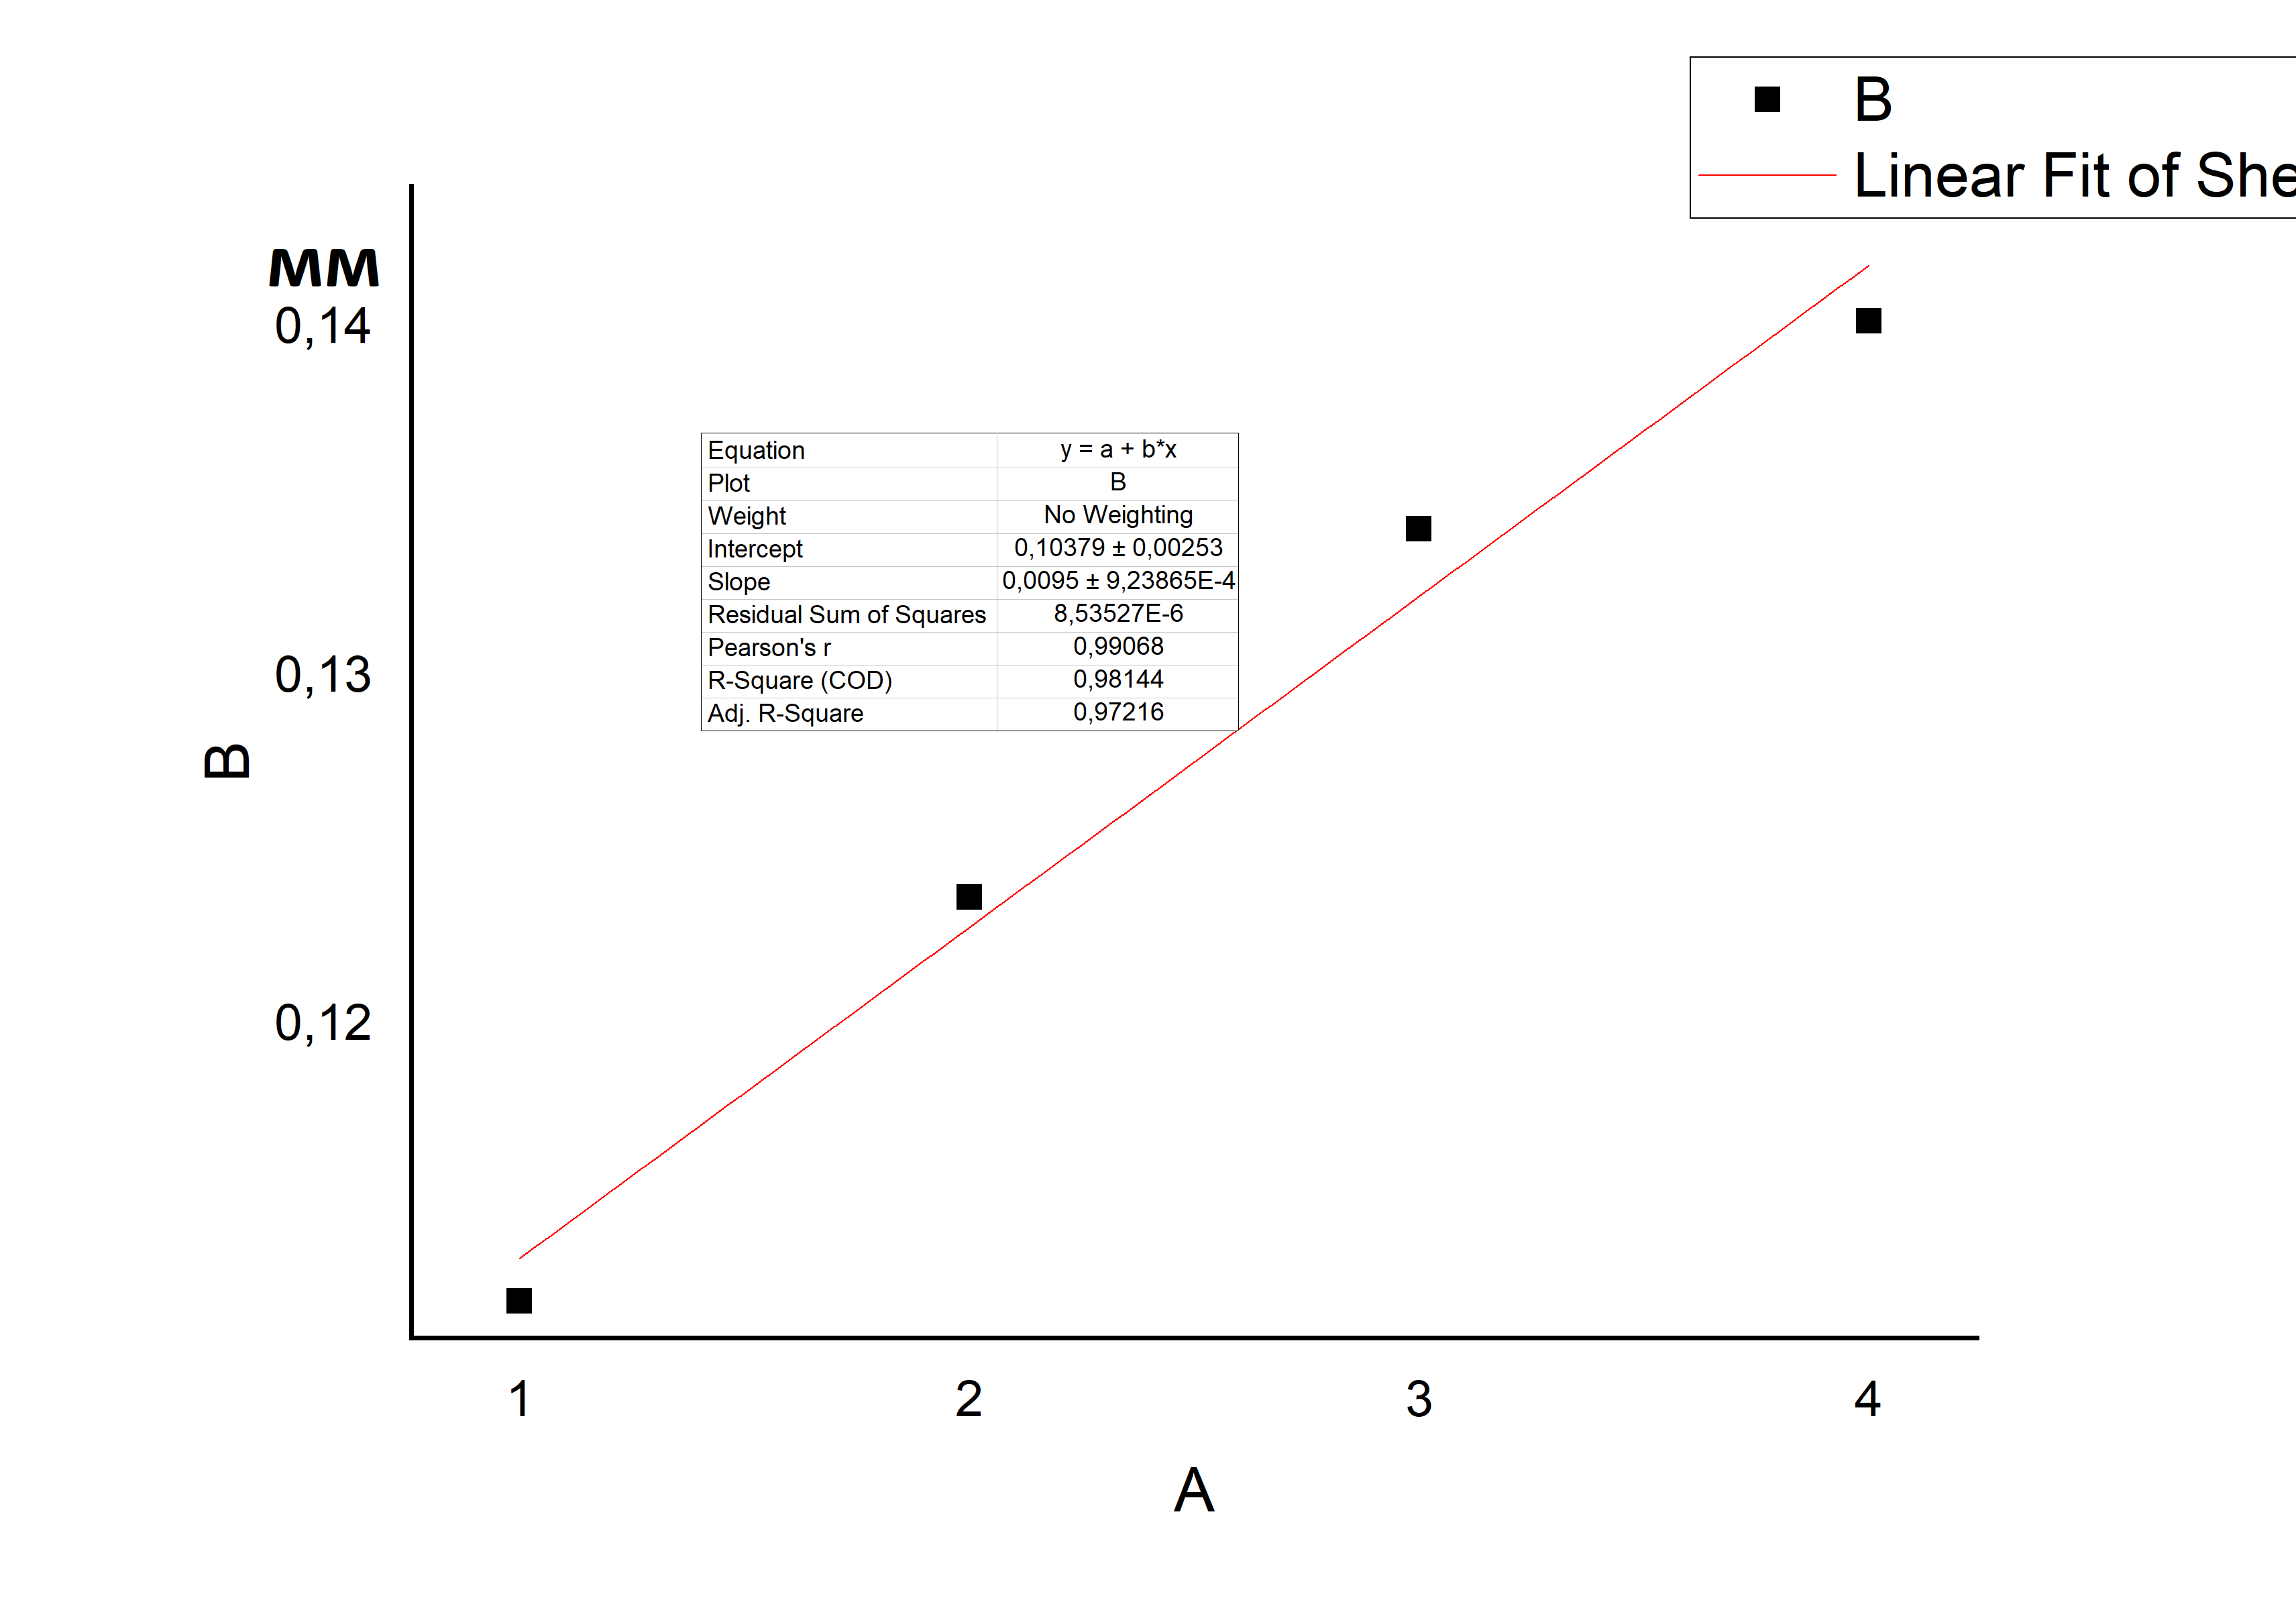
\includegraphics[scale = 0.4]{Рис1.png}}
 	\caption{График зависимости ширины зоны Френеля от ее номера}
 \end{figure}
 
 
 При измерении щели $S_2$ через микроскоп получается значение $b = 0,02 \cdot 16 = 0,32$ мм, что хорошо согласуется с измеренным значением $326$ мкм.
 
 В начале наблюдалась дифракционная картина с одной темной полоской. Далее, если увеличивать щель $S_2$, то количество темных полосок будет увеличиваться.
 
 Далее, вместо щели была установлена тонкая нить, микроскоп настроен на ее резкое изображение. При удалении микроскопа от нити количество наблюдаемых через микроскоп нитей начинает увеличиваться.
 
 \item Дифракция Фраунгофена на щели.
 
 При разгядывании дифракционной картины через микроскоп получим следующие значения:
 \begin{table}[h!]
 	\begin{center}
 	\begin{tabular}{|l|l|l|l|l|l|}
 		\hline
 	  $m$	& $-2$ & $-1$ & $0$ & $1$ & $2$ \\ \hline
 	  \text{мкм}& $-89$ & $-41$ & $0$ & $41$ & $82$ \\ \hline
 	\end{tabular}
 \end{center}
 \end{table}

 По этим данным строим график зависимости координат минимума от их номера:
 
 \begin{figure}[h!]
 	\center{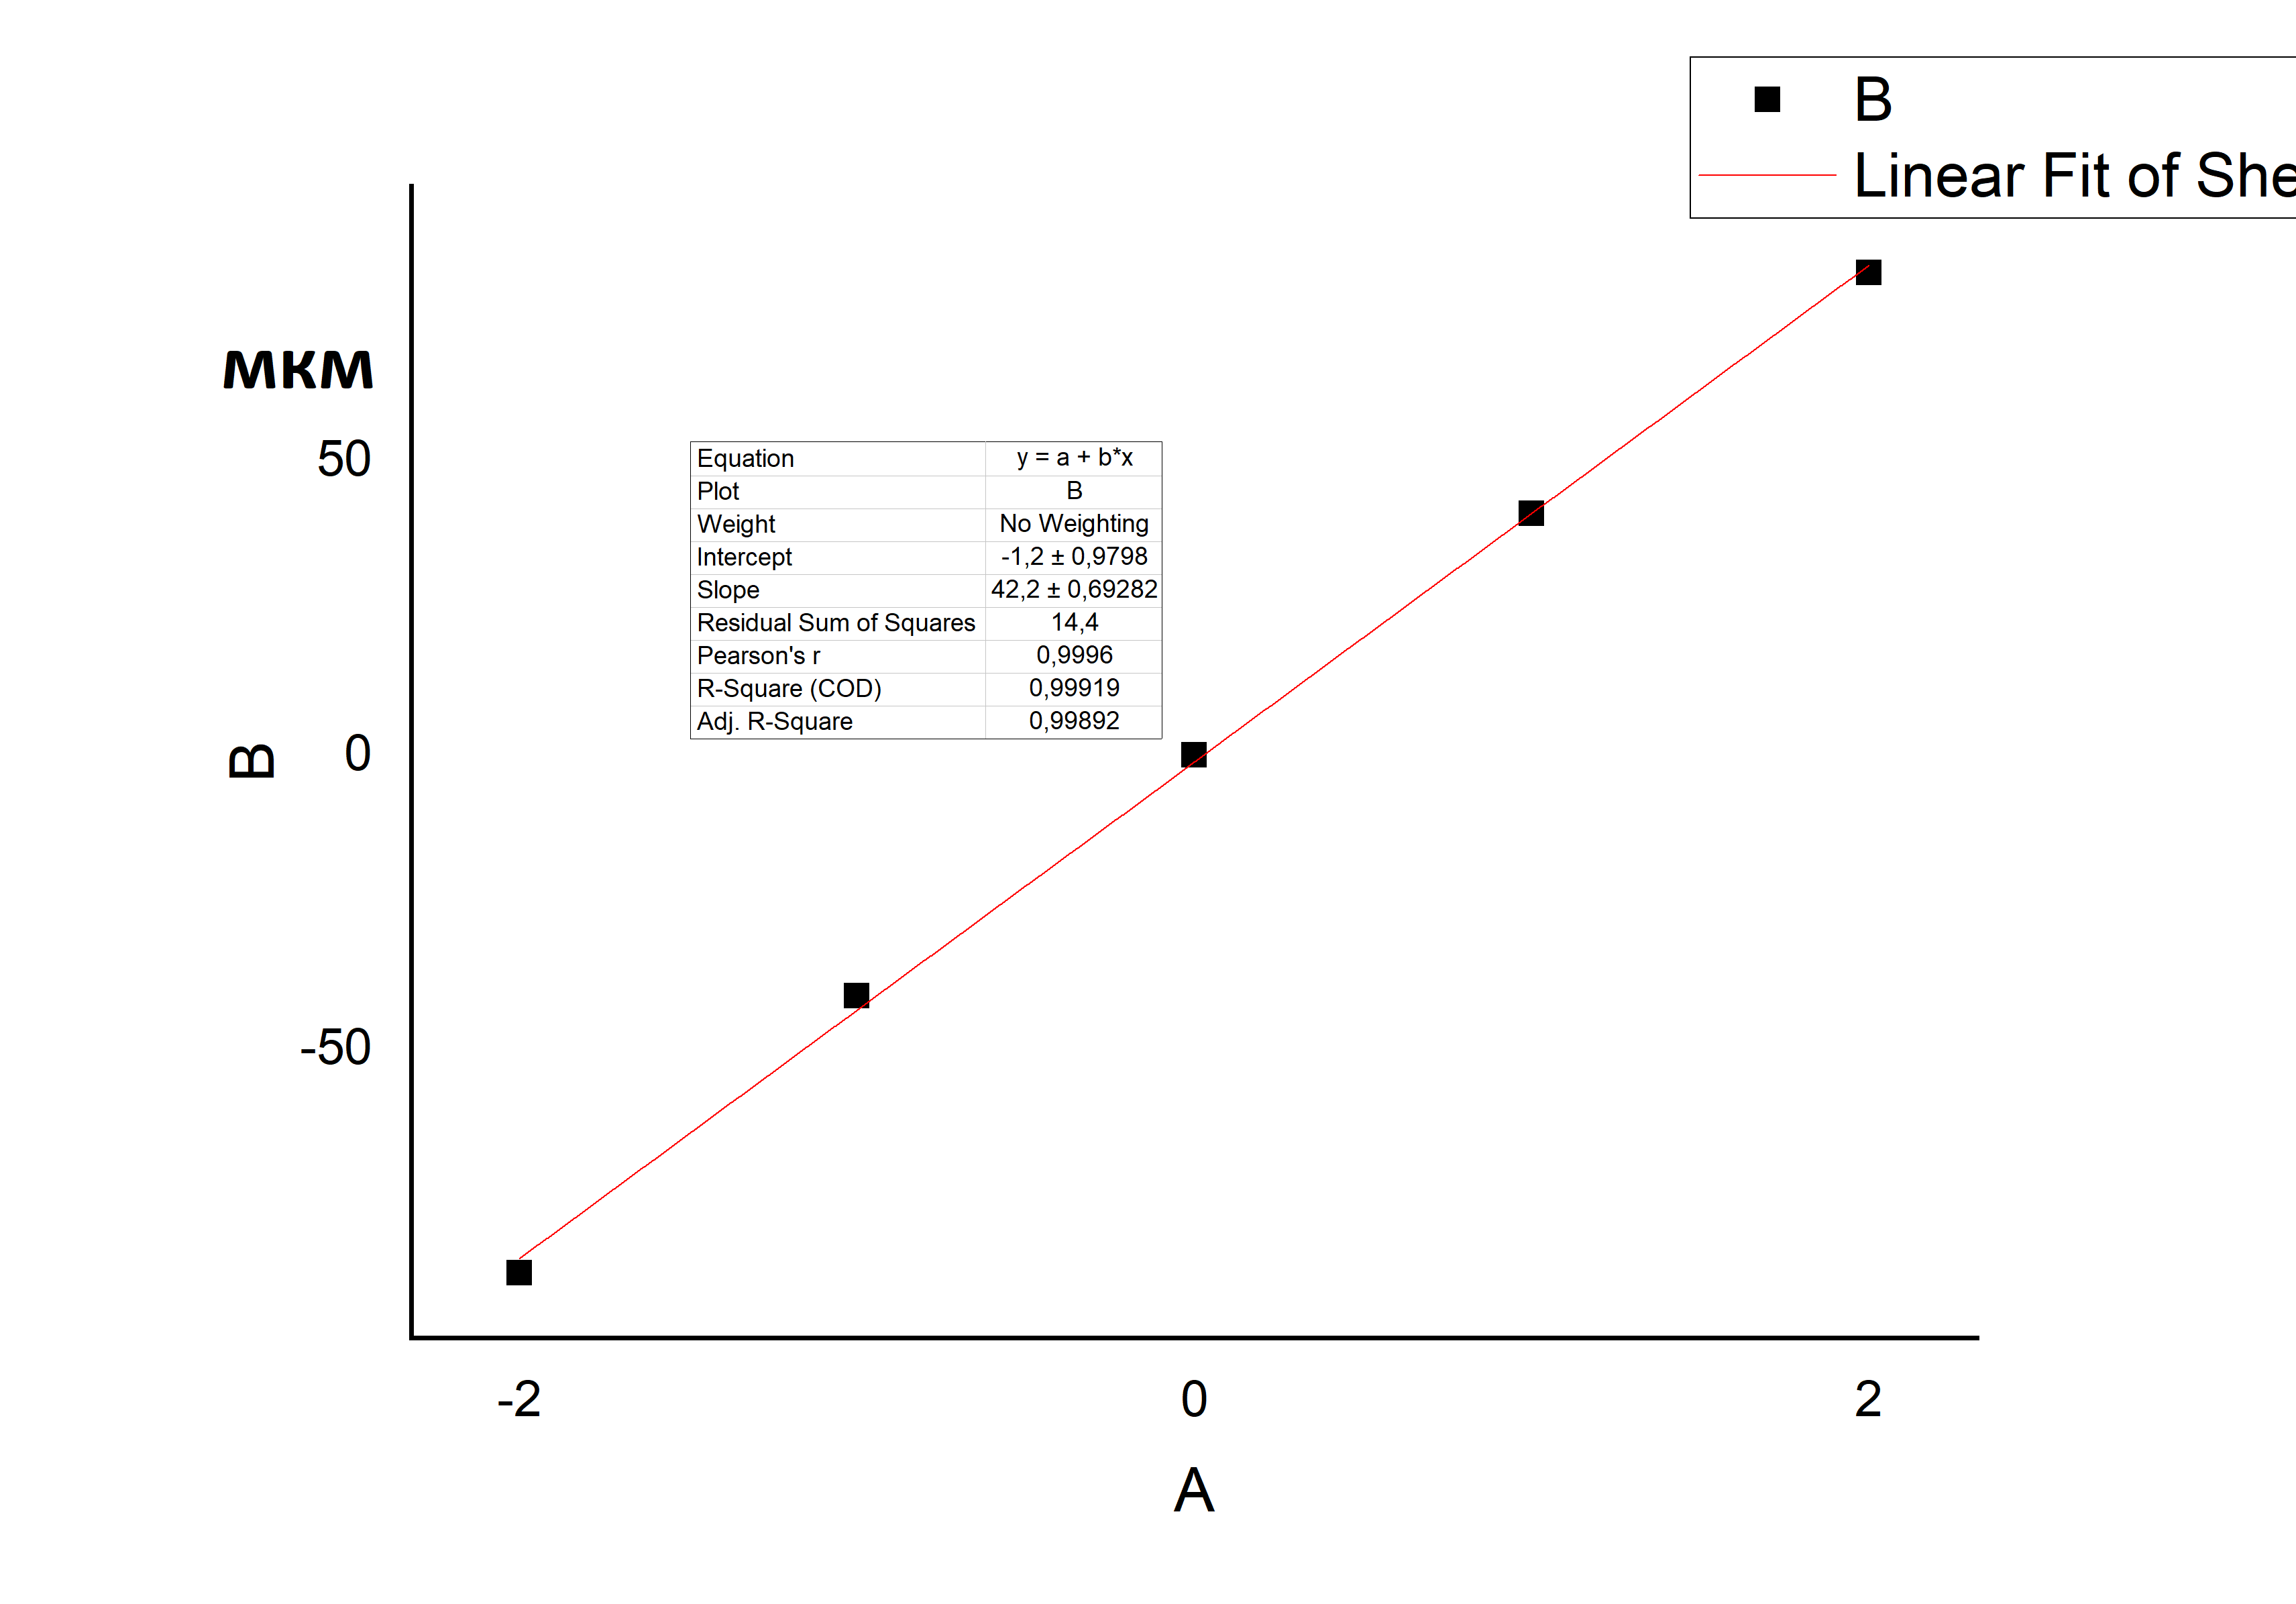
\includegraphics[scale = 0.4]{Рис2.png}}
 	\caption{График зависимости координат минимума от их номера}
 \end{figure}
 
 
 \item Дифракция Фраунгофена на двух щелях.
 $2,24$ мм - первый минимум. $3,68$ мм - последний минимум. Расстояние между минимумами - $1.44$ мм. Всего минимумов - 12, значит среднее расстояние между ними $0.12$ мм. Расстояния между краями максимумов - $0.08$ мм, откуда находим $d = f_2\frac{\lambda}{\delta x} =1.2$ мм. Из него получается рассчетное число максимумов $n =\frac{2d}{D}= 12$, совпадающее с экспериментальным.
 
 \item Влияние дифракции на разрешающую способность оптического инструмента.
 
 $D_{0\text{расч}} = \frac{\lambda f_1}{b} = 0.04 \pm 0.01$ мм. Измеренное значение равно 
 $D_{0\text{изм}} = 0.03$ мм - оно попадает в погрешность.
 
\end{enumerate}

\section{Вывод}
В работе исследовалась дифракция Фраунгофена и Френеля. Оказалось, что обе зависимости, рассматриваемые в работе, с большой точностью являются линейными, как и требует того теория. Было замечено, что количество темных полосок в первом эксперименте растет с увеличением ширины щели $S_2$.

Измеренное число максимумов $n=12$ совпало с вычисленным значением, также равны  $D_{0\text{расч}}$ и  $D_{0\text{изм}}$ в пределах погрешностей. Этот факт, а также подтверждение линейной зависимости ширины зоны Френеля и координат минимума от номеров показывает, что эксперимент поставлен удачно.
\end{document} % конец документа
 